\section{Additional Results}
\label{app:extra}
\begin{figure}[h]
\centering
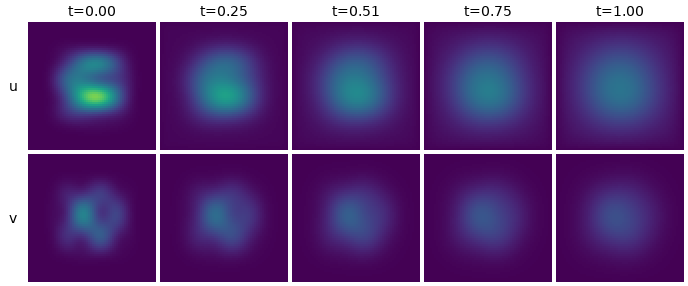
\includegraphics[width=0.62\textwidth]{figures/example_sheet.png}
\caption{A real image input: Gray--Scott, oscillation IC, zero Dirichlet BC, sample 1. Rows are the fields $u$ and $v$; columns are the five observed times. Every image uses this layout, colormap, and color range.}
\label{fig:example-sheet}
\end{figure}

\begin{table}[h]
\centering
\caption{Spearman correlation with $-D$ for each IC family (samples 0--9), and the range of similarities between different problems in the same family.}
\label{tab:perfamily}
\small
\begin{tabular}{llcccc}
\toprule
Model & Input & Bump & Oscill. & Patches & $S^{\mathrm{emb}}$ range \\
\midrule
EmbeddingGemma 2 & text & 0.24 & 0.17 & 0.24 & 0.985--0.999 \\
 & image & 0.72 & 0.78 & 0.77 & 0.997--1.000 \\
 & joint & 0.24 & 0.16 & 0.28 & 0.980--0.999 \\
Qwen3-VL-Emb.-2B & text & 0.37 & 0.50 & 0.44 & 0.898--0.996 \\
 & image & 0.83 & 0.80 & 0.72 & 0.987--0.999 \\
 & joint & 0.34 & 0.44 & 0.39 & 0.882--0.997 \\
GME-Qwen2-VL-2B & text & 0.47 & 0.42 & 0.48 & 0.973--0.998 \\
 & image & 0.87 & 0.83 & 0.81 & 0.985--0.999 \\
 & joint & 0.58 & 0.50 & 0.42 & 0.972--0.998 \\
\bottomrule
\end{tabular}
\end{table}

\begin{table}[h]
\centering
\caption{Exploratory (not planned in advance): average similarity between problems in the same IC family, grouped by what they share: the same equation with a different BC (9 pairs per family), the same BC with a different equation (45), or neither (99). The last row gives the average reference distance for the same groups (smaller means more similar).}
\label{tab:factors}
\small
\begin{tabular}{llccc}
\toprule
Model & Input & Same eq. & Same BC & Neither \\
\midrule
EmbeddingGemma 2 & text & 0.9971 & 0.9920 & 0.9896 \\
 & image & 0.9999 & 0.9989 & 0.9989 \\
 & joint & 0.9960 & 0.9930 & 0.9902 \\
Qwen3-VL-Emb.-2B & text & 0.9906 & 0.9513 & 0.9434 \\
 & image & 0.9983 & 0.9920 & 0.9920 \\
 & joint & 0.9923 & 0.9408 & 0.9368 \\
GME-Qwen2-VL-2B & text & 0.9968 & 0.9838 & 0.9812 \\
 & image & 0.9969 & 0.9899 & 0.9898 \\
 & joint & 0.9953 & 0.9835 & 0.9803 \\
\midrule
Reference $D$ & -- & 0.0019 & 0.0343 & 0.0343 \\
\bottomrule
\end{tabular}
\end{table}


\paragraph{Precision.}
As planned in the protocol, we re-encoded sample 0 of all 54 problems with EmbeddingGemma 2 in float32. The lowest cosine similarity between the float32 and bfloat16 embeddings of the same input is \precTextMinCos{} for text, \precImageMinCos{} for images, and \precBothMinCos{} for joint inputs. The two precisions rank pairs almost identically (mean Spearman correlation \precTextSS{}, \precImageSS{}, and \precBothSS{}). Agreement with the reference on this sample changes from \precTextRefB{} to \precTextRefA{} (text), from \precImageRefB{} to \precImageRefA{} (image), and from \precBothRefB{} to \precBothRefA{} (joint) when we switch from bfloat16 to float32. Reduced precision does not explain the results.
